%%--------------------Chapter 3------------------------
\documentclass[../UNBThesis2.tex]{subfiles}
\setlength{\parindent}{2em}
\begin{document}
\chapter{Literature Review}

short introduction describing the contents, the aim of the LR,

This Chapter 
Several data stream clustering algorithms have been implemented with the AP algorithm using different time window models. Out of all these algorithms, none of them implemented with a landmark time window model. Moreover, all these algorithms tested on synthetic and intrusion detection algorithms. There are no works that applied the stream AP algorithm on indoor localization data.


%To control which part of data is going to be processed, time window models have been proposed.
%New ideas continue evolving in data streams over time. Evolving needs updating data stream algorithms to adjust to the changes such as handle well rapid cluster evolution patterns.
%To handle and generate data in the stream mode, open-source frameworks for IoT data stream are being developed including MOA \cite{holmes2007moa}, Scikit-multiflow \cite{montiel2018scikit}, streamDM C++ \cite{bifet2017extremely} and Apache SAMOA \cite{de2013samoa}. THIS SHOULD BE MOVED TO LR

% K-medoids algorithm \cite{macqueen1967some} is a good strategy to find clusters easy and fast by randomly choosing K initial exemplars from data and assign closest data points to these exemplar as shown in figure \ref{medo}, these exemplar can be purify in the next steps. The only thing should be consider is the number of exemplars are not changeable but the algorithm maximize the size of similarities between exemplars and other objects. k-medoids algorithm requires to be run with a various random initialization to find a suitable exemplar but this works well when clusters are small.  
% \begin{figure}
% \centering
% \includegraphics[width = 11cm,height = 7cm]{image/Chapters/Chapter2/3.png}
% \caption{K-medoids greedy solution for toy dataset}
% \label{medo}%\cite{dueck2009affinity}
% \end{figure}




\section{Previous Research Work on Streaming AP }
% Using affinity propagation for streaming clustering faces two difficulties. First, AP has been implemented for batch processing but it should handle data clustering and large datasets in the online mode. The most important point to consider is AP suffers from quadratic computational complexity.
Extensive data that are continuously coming are required to store. Analyzing big datasets and extracting patterns is not possible with affinity propagation due to the time complexity issue.
One way to apply affinity propagation algorithm is using the divide and conquer approach \cite{khalilian2016data}. This approach introduced by Nittel et al.\cite{nittel2004scaling}, has mainly three steps as shown in Figure \ref{dividee}: partitioning the dataset into different chunks, then clustering each chunk and find the results, lastly, computes the results out of all chunks of data. 

\begin{figure}[!h]
    \centering
    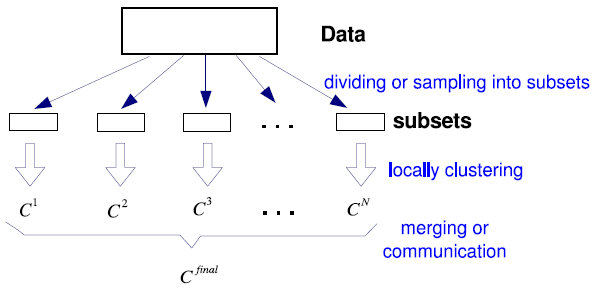
\includegraphics[width = 11 cm]{image/Chapters/Chapter3/divide.PNG}
    \caption{Divide and conquer approach to generate clustering out of big data \protect\cite{zhang2009toward}}
    \label{dividee}
\end{figure}


Our first attempt working with the extensive dataset was to implement this technique to generate data stream clustering \cite{ivarispatio}, and it was the first version of DSAP, which is presented in this thesis. However, it has a history of all data points, and the time and memory complexity are still high, and most algorithms that have this approach are unable to track the change in the trend of the data stream. 
Due to the reason above, some research has been done on AP streaming clustering and introduce new approaches.

%Elmi
% It must be emphasized that both Divide-and-Conquer and two-level schemes keep their computational load
% within reasonable limits as they only build the data model upon the users explicit request. In the rest of time, they only maintain a summary of the data, which makes them ill-suited to applications such as system monitoring where the data model has to be continuously available at all times.


There are a few algorithms are introduced based on AP algorithm for data stream clustering and they are shown in Table \ref{APCLU}. 


\begin{table}[!h]
    \centering
    \caption{Overview of data stream clustering algorithm based on AP. }
    \label{APCLU}
    \small
    \begin{tabular}{c c c c c}
    \hline
      \textbf{Algorithms} & \textbf{Year} & \textbf{ Method } & \textbf{Processing} & \textbf{Time window model}\\
     \hline \midrule
     STRAP                &   2008        &    AP             &    Online          & Sliding \\
     \hline 
     IStrAP               &   2012        &    AP             &    Online          & Sliding \\
    \hline
     APDenStream          &   2013        &    AP             &     Online-offline & Pyramidal(offline)   \\
     \hline
     SSAPStream           &   2015        &    AP             &     Online         &   Damped    \\
    \hline
     SED-Stream-AP        &   2018        &    AP             &    Online-offline   & Damped(offline)\\
     \hline
     ISTRAP               &   2018        &    AP             &   Online           & - \\
\bottomrule
    \end{tabular}
\end{table}

% The other improvement of AP to handle huge datasets was WAP or weighted AP \cite{zhang2009toward}. Under the premise of not changing the amount of passed information, this algorithm integrates the neighboring points, making the integrated points have the same clustering results with the original points.
% , zhang2013data
\begin{itemize}[leftmargin=*]

\item[]\textbf{STRAP Algorithm}

In 2008, Zhang et al. \cite{zhang2008data} proposed streaming AP called STRAP, extending affinity propagation for data stream clustering. 
This model is inspired by DBSCAN and DenStream introduced in Chapter Background. STRAP is built of several steps. 
The first step is weighted AP to handle duplicated objects without losing performance.
Second, hierarchical WAP, dealing with quadratic AP complexity and reduce it by utilizing AP on subsets of data and then utilizing Weighted AP on the exemplars obtained from subsets.
Eventually, with online clustering, STRAP extends Hierarchical WAP to deal with changes in the data distribution by updating exemplars and storing the outliers. As illustrated in Figure \ref{stmodl}, STRAP involves four main steps as follow: 


\begin{itemize}
    \item[$\bullet$] AP applied to the first bunch of data to computes the first centroids and initialized the streaming model.
    \item[$\bullet$] As the stream comes into the model, each data point $x_t$ is compared to the centroids $e_i$. This comparison is based on the Euclidean distance of $x_t$, $e_i$ with the threshold $\epsilon$, which is heuristically set, and the value is equal to the average distance between data points and centroids in the initial model. If $x_t$ is far from the nearest centroid, it goes to the reservoir. If not, $x_t$ is assigned to the ith cluster, and the STRAP will be updated accordingly. STRAP has a mechanism to forget old centroids which they have not been visited for some time and to keep them in control.
    \item[$\bullet$]  Two restart procedures have been used in STRAP. First, if the number of outliers in the reservoir exceeds the reservoir's size, the restart criterion will be triggered. Second, it is related to the distribution of the data points by applying Page-Hinkley (PH) test and detect the changing trend of data points. 
    \item[$\bullet$] If restart criterion called by either fill up the reservoir size or the PH test, model is rebuilt by launching WAP algorithm from current centroids and reservoir.
\end{itemize}

\begin{figure}
\centering
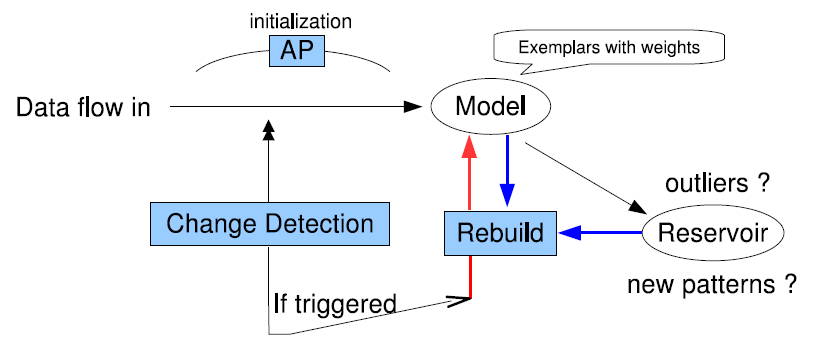
\includegraphics[width = 13 cm]{image/Chapters/Chapter3/strapmodel.PNG}
\caption{The framework of STRAP algorithm. }
\label{stmodl}
\end{figure}



% To validate a STRAP, the Intrusion Detection benchmark(KDD99) and EGEE real-world datasets are used for monitoring and discovering anomalies within a grid computing infrastructure. The result of this work is compared with DenStream, and comparatively satisfactory results are investigated. Also, computational time in this model is higher than DenStream. 


The proposed STRAP algorithm was analyzed on guaranteeing acceptable distortion loss when exemplars slightly drift from the already selected ones, with a small amount of memory and computing time. The performance of STRAP in clustering quality and efficiency is validated on the KDD’99 dataset and the URLs stream. However, STRAP improves clustering purity rather than DenStream, and computational time is also higher than the DenStream algorithm. In addition, STRAP is a model for the stream at any time, whereas DenStream only builds the model upon request. The validation on URLs stream also demonstrates that STRAP achieves very high accuracy and purity for collecting malicious URLs.




% % From APDENSTREAM:
% This algorithm can determine
% the number of clusters automatically and detect the real-time
% changes of the data stream at the same time. However, the
% clustering quality depends on the size of the sliding window.
% Meanwhile, it is not considering how the arrival time will
% affect the clustering results. The clustering effect is not
% satis factory when noises are too much




\item[]\textbf{IStrAP Algorithm}

IStrAP \cite{li2012improved} is an improved version of the STRAP algorithm to meliorating the efficiency of this algorithm. STRAP algorithm frequently applies the WAP algorithm to combine the initial clustering results with the reservoir’s data points to re-cluster in a fast manner. Clustering is sometimes ineffective due to the handling of outliers well in the reservoir. To improve the efficiency of clustering results, they introduced a method to remove outliers. This method is based on the statistical properties of the window data. The outlier refers to the abnormal behavior deviating from the normal value. Such data may be generated in emergency situations or generated when an error occurs. The process of removing outliers is consists of four steps. 
\begin{itemize}
    \item[$\bullet$]  The reservoir statistics (maximum value, minimum value, sum and average value) from received stream data are obtained.
    \item[$\bullet$] Standard deviation of data points in the reservoir are computed.
    \item[$\bullet$] The sampling parameter ($\sigma$) needs to be set. This parameter can reflect the distribution of the data in the window. The $\sigma$ value is standard deviation of the data.
    \item[$\bullet$] Outliers are being removed if they are outside of the interval equal to [Avg-$\sigma$, Avg + $\sigma$].
\end{itemize}

 

IStrAP used KDD Cup 99 dataset and used the Page-Hinkley standard test to update the clustering model. The results show that the IStrAP has higher accuracy, lower time complexity, and better adaptability for stream data over than STRAP. With this dataset, they just chose 120 data points to show the result, and the result is poorly demonstrated with the percent of accuracy and time.


\item[]\textbf{APDenStream Algorithm:}

Zhang et al. \cite{zhang2013online} proposed a data stream clustering based on AP and density methods to improve the STRAP model's accuracy and timeliness in a noisy environment. This algorithm applies two-phase clustering, online and offline approaches. The online phase detects data distribution changes of the new data points, updates the micro-cluster decay density, and generates real-time results. The offline, which invoke by the user, choose a specific time frame by applying a pyramidal time window model and gives final query results. The process of this work is depicted in Figure \ref{APden}. 


\begin{figure}[h]
\centering
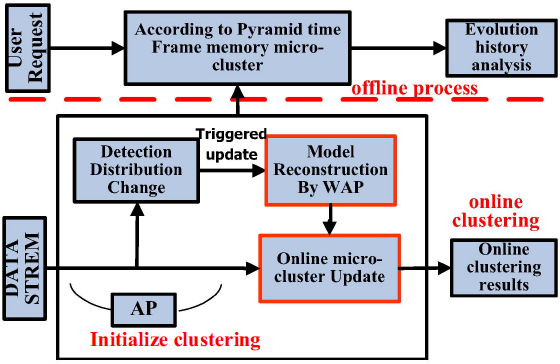
\includegraphics[width = 10 cm]{image/Chapters/Chapter3/APDenstream.PNG}
\caption{APDenStream clustering model introduced by Zhang in 2013. }
\label{APden}
\end{figure}


The overall APDenStream algorithm can be explained as follow:

\begin{itemize}
    \item[$\bullet$] AP algorithm is applied to the first $InitN$ points $P$ to initialize the online process. The first group of micro-clusters $mc$ are obtained by scanning $P$. If the micro-cluster density of the micro-cluster $mc$ is greater than the threshold $D$, it is labeled as a dense micro-cluster, and the average radius of all dense micro-clusters is being chosen as an initial radius $\epsilon$.
    
    \item[$\bullet$] The new point comes into the model, and it places to its nearest dense or sparse micro-cluster. If it cannot absorb any cluster, it goes to the reservoir. Then the model will be updated. As time passes, the number of micro-clusters and sparse micro-clusters is increased. To keep the clusters in a limited number and avoid memory issue, a dynamic online maintenance strategy is being used.  This strategy consists of two-part. One is for checking each dense micro-cluster every time period in order to determine whether to remove it. The other one is when the number of sparse micro-clusters is increasing by checking the minimum weight limit of sparse micro-clusters. 

    \item[$\bullet$] Whenever the reservoir is full, the model will rebuild, and new clusters will add to the model by applying the WAP algorithm.     
    
   \item[$\bullet$] The last step is offline processing which can master a depth-first traversal to find dense micro-clusters by the snapshot of the moment, and the more accurate micro-cluster is formed. Also, snapshot at time $t_c$ and time $t_ch$ can be found in the pyramidal time frames according to the current time $t_c$ and user-specific time range $h$. 
\end{itemize}



The experimental dataset used is KDDCUP'99, network intrusion detection with the 494020 TCP connection belongs to 23 networks. The results show that the APDenStream is more accurate than the STRAP algorithm due to the proposed summary data structure and benefited from its online elimination strategy, which maintains the potential micro-clusters in the stream in the time of removal of outlier noise point.
Also, APDenStream can remove outliers without upgrade potential noise points timely, while STRAP historical expired micro-cluster is taken into account.


% it is a good paper related to threshod, a metric for data distribution --> old DSAP with 2 threshold

\item[]\textbf{SSAPStream Algorithm:}

Atwa and Li \cite{atwa2015affinity} proposed a semi-supervised algorithm, an extended AP called SSAPStream, to handle evolving data streams over the online phase. This method is semi-supervised aims to improve the performance by learning from a combination of both labeled samples and unlabeled data. For a certain labeled data point, $x_i$ and unlabeled data point $x_j$, two possible situations may occur where the labeled data point may be associated with the unlabeled data point after ruining the AP algorithm. One is unlabeled data point $x_j$ takes the labeled point $x_i$ as a cluster centroids, and the other one is the labeled $x_i$ takes the unlabeled $x_j$ as a cluster centroids. If one of these two conditions happens, the unlabeled $x_j$ is the most similar to the label $x_i$. Then, the unlabeled $x_j$ is selected and set to the label of $x_i$. This process will repeat until all unlabeled data points finish.
They considered that the problem of data stream clustering with the damped time window model then the weight of data points $x_i$, decrease with time $t_k$ and calculated by decay function:

\begin{equation}
    w(x_i, t_k) = 2^{\lambda(t_k - t_i)}
\end{equation}

The proposed algorithm involves three main steps:
\begin{itemize}
    \item[$\bullet$] Apply AP algorithm on the first bunch of data at time $t_0$ to initialize the model.
    \item[$\bullet$] As a new data point flows into the model, it compares with the existing centroids based on the heuristic threshold; if too far from the nearest centroid, it goes to the buffer, or if it is far, the model will be updated. The threshold $\epsilon$ is set to the average distance between data points and centroids in the initial model.
    \item[$\bullet$] If a buffer is full or a change in the stream is detected, the model is rebuilt, and buffer 
    \item[$\bullet$] To prevent the number of centroids goes beyond the control, old ones should be removed. For each centroid, if not any new data point is merged, the weight of the centroid will decay gradually, and it should be deleted.
    \item[$\bullet$] In order to detect changes in the model, an exemplar variation threshold $\delta$ is introduced to determine if the ratio of data points associated with the centroids is big enough. If the centroid that exceeds $\delta$ is seen as a new cluster centroid. Then, the number of centroids is counted, and the ratio of different these centroids is compared with the new threshold $\phi$. If the ratio of different centroids is larger than the threshold $\phi$, many centroids are varied in the ratio of data items, then the model should be updated.
\end{itemize}


To evaluate the effectiveness and efficiency of the algorithm, two real and two synthetic datasets are used. Two real datasets are KDDCUP99 and URLs. KDDCUP99 contains a range of TCP connection records of LAN network traffic. The URLs dataset is used to predict malicious URLs from good ones.
The SSAPStream algorithm results are compared with the StreamKM++, DenStream, CluStream, and STrap. The output shows that these algorithms have advantages over other algorithms in memory usage except the StreamKM++. 
To set threshold parameters, they suggested finding the data distribution changes that are not easy for many streaming data. 


\item[]\textbf{SED-Stream-AP Algorithm:}


The other stream clustering approach based on the online and offline process is called SED-Stream-AP \cite{sunmood2018evolution}, Based on the evolution-based clustering of SED-Stream, which is able to support the evolution of clustering such as appearance, disappearance, self-evolution, merge and split. The. In the online phase, SED-Stream-AP is able to detect evolving clustering structures, which are cluster appearance, disappearance, self-evolution, merge, and split. During the offline phase, the AP algorithm is adopted to find the final clustering results. The algorithm flowchart is illustrated in Figure \ref{sed}.

\begin{figure}
\centering
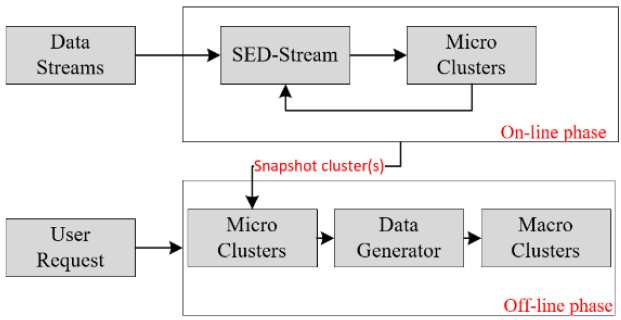
\includegraphics[width =10 cm]{image/Chapters/Chapter3/sed.PNG}
\caption{The framework of SED-Stream-AP algorithm.}
\label{sed}
\end{figure}


The online phase of the SED-Stream-AP algorithm is formed with different steps. First, when a new data point flows into the model, existing clusters in the SED-Stream-AP fade by decay function. Then, based on the splitting and merging features, the algorithm splits and merges the potential clusters if they are needed. Next, if any new cluster appears, it is considered as an active cluster. Lastly, the incoming data point is assigned to the closest cluster.  Otherwise, it creates its 1-element cluster. Specifically, cluster split is based on the distribution of dimension values summarized by the cluster’s histogram.
If a statistically significant valley is found between two peaks in the histogram’s value along dimensions, the cluster splits. 

The offline phase operates with the user request and consists of three steps. 
\begin{itemize}
    \item[$\bullet$] Retrieves micro-clusters have been obtained from the online phase by using FCH (Fading Cluster Structure with Histogram), a data structure that keeps representations of all the micro-clusters.
    \item[$\bullet$] Generates new data points only selected dimension from the online phase using cluster representations. The number of data points to be generated is defined based on the weight of the online phase micro-clusters
    \item[$\bullet$] calculates macro-clusters using the affinity-propagation clustering algorithm.
\end{itemize}


The SED-Stream-AP algorithm is evaluated by six different datasets, which are KDDCUP'99, forest covertype, Statlog, breast cancer Wisconsin, electricity, and synthetic datasets. 



\item[]\textbf{ISTRAP Algorithm:}

Another work on AP streaming clustering is ISTRAP \cite{sui2018dynamic}. ISTRAP is an improved model of STRAP which has been introduced in 2018. This model which inherits advantages of STRAP algorithm, gains better performance in terms of cluster evolution. This algorithm can detects three types of evolution patterns: emergence, disappearance, and re-occurrence which STRAP can handle the first one and the next two types are implemented in this work. Cluster emergence refers to the occurrence of a new cluster at time $t$. Cluster disappearance refers to the existing cluster that is not visited by the recently arrived data
points. Disappeared clusters need to be removed from the model. Cluster re-occurrence defines where a previously disappeared cluster recurs at time $t$.

For this algorithm, two reservoirs are introduced: one is the for saving the outliers (emergence) and the second one is for storing inactive clusters (re-occurence). Also, ISTRAP defines the clusters into two states, active and inactive, at each timestamp. Active state means that the cluster is still valid at current timestamp because at least one data point is assigned to it during a time interval. Inactive state indicates the corresponding clusters are expired because they are out of recent data point which representation for any pattern of the data.
the framework of the ISTRAP algorithm is illustrated in figure \ref{istrap} which is described as below:

\begin{figure}
\centering
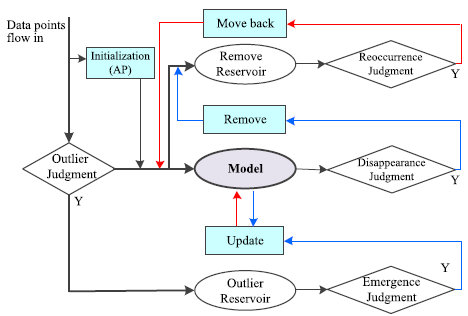
\includegraphics[width =10 cm]{image/Chapters/Chapter3/istrap1.PNG}
\caption{The framework of ISTRAP algorithm.}
\label{istrap}
\end{figure}

\begin{itemize}
    \item[$\bullet$] First, initial exemplars are obtained by applying the AP algorithm on the first bunch of data.
    \item[$\bullet$] As the stream flows in, each data point will go the outlier judgment step, and the minimum distance of the data point from the exemplar compares with the threshold. If it is less than the threshold, it will assign to the nearest exemplar; otherwise, it goes to the reservoir.
    \item[$\bullet$] All clusters in remove reservoir are checked if they re-occur, then recurrent clusters will be moved back into the model
    \item[$\bullet$] The emergence criterion is triggered if new clusters need to be obtained. So, from the outlier reservoir, the model will be rebuilt by the WAP algorithm.
    \item[$\bullet$] The model will check all active clusters if they are still active or not. The inactive clusters will be removed and goes to the removed reservoir.
\end{itemize}

The clustering quality of this algorithm depends on mostly four parameters that need to be chosen carefully, such as $\delta$, $\alpha$, $\beta$, $\lambda$. The effect of three forms of evolution by controlling the number of outliers or $\delta$. The threshold for emergence detection is defined by $\alpha$, and it affects the stability and processing time of the algorithm. The maximal duration tolerance or $\beta$ means an active cluster is not visited by new data points. Larger $\beta$ means less possibility that clusters are inactive. The last parameter $\lambda$ represents the minimum number of data points assigned if recurrent clusters have to be sent to the model, and if $\lambda$ is small, it means more recurrent clusters are detected. 

Four Real datasets and two artificial numerical datasets are applied to evaluate this algorithm. The real-world data stream,  MNIST, contains handwritten digits from 0 to 9 and is used to test the performance of the ISTRAP. In the end, the results compared with the STRAP algorithm and find out that STRAP is unable to detect re-occurrence. However, ISTRAP has very powerful effectiveness in tracking the re-occurrence of the with a delay.







% \section{K-means Stream Clustering}
% For scalable and low-complexity way of transferring data from network to the mobile phones \ref{cramariuc2016clustering}.




%%%%##########  FOR now -- uncomment 
% \section{Data Stream Clustering}

% To perform data stream clustering to access and see the data over the time many data stream clustering algorithm have been introduce.
% CluStream \cite{chen2007density} is online and offline framework for clustering dynamic streaming data. This algorithm uses Pyramidal time window that allow micro-clusters to split and merge over time. Online phase, is sampling process of the $k$ desired clusters and this $k$ clusters are emitted at chosen time intervals, through some off-line clustering method.


% A common baseline algorithm for streaming clustering, is streaming k-Means \cite{ailon2009streaming, braverman2011streaming} uses its update process from the Lloyd algorithm. However, similar to CluStream, micro-clusters is maintained in online phase, to be further clustered in an off-line step. Similar to K-means, streaming K-means has the same process for assigning incoming data points to the nearest representative cluster. The value for having $k$ number of cluster is not available, and this can be done with some sort of inter-cluster similarity or intra-cluster dissimilarity metric. the main drawback of streaming k-Means is that it is highly dependent on the input order of the data stream.

\end{itemize}

%any streaming algo for indoor

\todo[inline]{research premise}
There First group is partitioning data stream clustering algorithm which they are listed in Table \ref{landmarkwin}. As far as we had research, there is not any research work present with affinity propagation used landmark time window model.

There is no paper related to occupant behaviour(stair usage) + stream clustering???
There is no paper related to ecounter(sensors) + clustering as well as stream clustering????

paper related to people counter+ clustering ????

Several data stream clustering algorithms have been implemented with the AP algorithm using different time window models. Out of all these algorithms, none of them implemented with a landmark time window model. Moreover, all these algorithms tested on synthetic and intrusion detection algorithms. There are few works that applied the AP algorithm on indoor localization data. _>> to be used for conclusions


% \section{occupancy}
%\section{Latest Development in Indoor Localization }

PAPER'S BELOW SHOULD BE MOVED TO THE PREVIOUS METHODS


The people’s counting is a very important topic to design any system for behavioral analysis. It is used to measure and manage people’s behaviour within area.

Using stairs and monitor human activity in the building is one scenario for indoor localization and behaviour analysis.


%Carbonare et al. \cite{carbonare2018clustering} uses clustering method to investigate the occupant behaviour and their pattern in residential buildings. Two clustering method have been used: Whole time series and feature clustering with the K-means and these features are window opening and indoor temperature. The results show that feature selection has a better output than time series clustering. ?????
   


%There are many works dealing with the indoor localization problem by using WLAN-based techniques.
Clustering method could efficiently reduce computational complexity and memory requirements in large fingerprinting localization data to train ANN model. K-means clustering algorithm is one of these algorithm which is easy to implement with low time complexity. However, this algorithm is starts with an initial guess as a number of clusters, which is in the condition of close to the true solution to avoid local minima. Selection of such a starting point is not easy. Also, it would affect the location accuracy performance \cite{das2007automatic, ding2013fingerprinting}.

Genming et al. \cite{ding2013fingerprinting} introduces a fingerprinting-based localization algorithm using affinity propagation in conjunction with neural network. 
This model consists of two stage offline and online. The offline stage applies clustering and ANN training on the data. First,  a set of RSS from N available access point is collected and stored in the database. AP clustering algorithm is used in this part to to reduce the computation cost and memory of the system and partitions the reference points into different clusters represents by centroids. After clustering, the training of artificial neural network is carried out for each cluster.
The online stage, the unknown location is obtained by in two steps. First, by applying pattern matching to calculate the similarity between the new collected signal and cluster centroids and then choose sets of best match clusters for the next ANN localization phase.

Xuke et al. \cite{hu2015improving} proposes an improved WiFi fingerprinting positioning algorithm called WKNN-SAP. First, a new fingerprint distance estimation using RSS distances and access points similarities is used. Then, semi-supervised AP clustering algorithm is applied to find isolated points and remove them to have a reasonable clustering output and eliminate some outliers.

On the other hand, they applied K-means algorithm to compared both clustering results to improve the localization accuracy. and they figured out that while AP outperforms Kmeans in both the accuracy improvement and stability and this is because AP algorithm is less affected by the clustering number. Moreover, proposed fingerprint distance model can better adapt to the indoor environment with distinct access points.

%Existing stream clustering algorithms often have issues regarding asymptotic scalability [3], dimensionality limits [4] and robustness to noise





Lee et al. \cite{carraher2016random} introduces streamingRPHash is motivated by
a particularly difficult case in Nearest Neighbor, a method for clustering high-dimensional data streams to solve the other clustering problem on streaming data by applying two real world dataset, ujIIndoorLoc and ‘Human Activity Recognition datasets.
For UjIIndoorLoc data, based on the 520 of signal strength intensity, building ID is used as the target variable which has three possible values related to each building.
Human Activity Recognition datasets has 561 attributes representing time and frequency domain variables.
the result of the proposed algorithm is compared with the streaming K-means, and DSt algorithms and it shows that their proposed algorithm and streaming K-means have the same results in term of run-time and memory requirement but with increase the dimension, streamingRPHash has a better result.



To the best of our knowledge, streaming AP models have not yet been applied for any people counting data streams.  

 STILL TO FIND OUT THE RESEARCH PREMISES: WHY ARE POUR APPROACH MOST SUITABALE FOR CLUSTERING INDOORL LOCATION DATA STREAMS..


Data stream affinity propagation algorithm has been chosen for indoor localization data in this research work. For this algorithm, every data point is an exemplar, and it means they have equal importance and there is no prior reason for preferring one observation over another one. Also, the AP algorithm does not require the number of clusters as an input which makes our work more robust, especially if it uses for the cloud side. AP's main issue is the computation efficiency that we make it possible by applying the time window model and making it a stream. This algorithm is applied in many scientific research and different datasets such as intrusion detection, energy, gene expression, psychology, business, physical science, social science, etc. However, to the best of our knowledge AP model has not yet been applied for any people counting data and streaming AP for any indoor localization dataset.

K-means algorithm is one of the most common methods for clustering distance-based objects that we have applied for our data. However, this method is less effective, or even inapplicable, for the application we used. For example, K-means results find cluster centroids between locations which does not make sense for our interpretation. 


%  affinity propagation can be used to cluster objects measured on non‐distance‐based similarity measures that arise in psychology, such as those obtained from stimulus recognition or paired comparison tasks (see, for example, Hubert, Arabie, & Meulman,






\end{document}